\documentclass[a4paper,11pt]{article}
\usepackage[top=2cm,bottom=2cm,left=2cm,right=2cm]{geometry}
\usepackage[utf8]{inputenc}
\usepackage[frenchb]{babel}

\usepackage{multirow}
\usepackage{makecell}
\usepackage{fancyhdr}
\usepackage{caption}
\usepackage[final]{pdfpages}
\usepackage{tikz,pgfplots,pgf}
\usepackage{subcaption}
\usepackage{siunitx}
\usepackage[toc,page]{appendix}
\usepackage{tcolorbox, listings} 
\usepackage{sectsty}
\usepackage[french]{minitoc} 
\usepackage{hyperref}
\usepackage{colortbl}
\usepackage{mwe}
\usepackage{amsmath}

\definecolor{Pantone2377C}{HTML}{2C5574}
\definecolor{subtitlecolour}{HTML}{00A2A9}
\definecolor{codegreen}{rgb}{0,0.6,0}
\definecolor{codegray}{rgb}{0.5,0.5,0.5}
\definecolor{codeblue}{HTML}{3E8BC0}
\definecolor{codeorange}{HTML}{ffa334}
\definecolor{backcolour}{HTML}{efefef}

\lstdefinestyle{myPython}{
    language=Python,
    backgroundcolor=\color{backcolour},   
    commentstyle=\color{codegreen},
    otherkeywords={plt, np, df},
    keywordstyle=\color{codeblue},
    numberstyle=\tiny\color{codegray},
    stringstyle=\color{codeorange},
    basicstyle=\ttfamily\footnotesize,
    breakatwhitespace=false,         
    breaklines=true,                 
    keepspaces=true,                 
    numbers=left,       
    numbersep=5pt,                  
    showspaces=false,                
    showstringspaces=false,
    showtabs=false,                  
    tabsize=2,
}

\lstdefinestyle{myLog}{
    language={[latex]TeX},
    backgroundcolor=\color{backcolour},   
    basicstyle=\ttfamily\footnotesize,
    breakatwhitespace=false,         
    breaklines=true,                 
    keepspaces=true,                 
    numbers=left,       
    numbersep=5pt,                  
    showspaces=false,                
    showstringspaces=false,
    showtabs=false,                  
    tabsize=2,
}

\lstset{
  backgroundcolor=\color{backgroundColour},   
  commentstyle=\color{codegreen},
  keywordstyle=\color{codeblue},
  numberstyle=\tiny\color{codegray},
  stringstyle=\color{codeorange},
  basicstyle=\footnotesize,
  breakatwhitespace=false,         
  breaklines=true,                 
  captionpos=b,                    
  keepspaces=true,                 
  numbers=left,                    
  numbersep=5pt,                  
  showspaces=false,                
  showstringspaces=false,
  showtabs=false,                  
  tabsize=2,
  literate=
  {é}{{\'e}}1
  {è}{{\`{e}}}1
  {ê}{{\^{e}}}1
  {û}{{\^{u}}}1
  {ù}{{\`{u}}}1
  {â}{{\^{a}}}1
  {à}{{\`{a}}}1
  {ç}{{\c{c}}}1
  {Ç}{{\c{C}}}1
  {ô}{{\^{o}}}1
}


% Entête et pied de page
\pagestyle{fancy}
\rhead{
\includegraphics [scale=0.035]{img/ensta-logo.png}}
\chead{}
\lhead{}
\lfoot{Tanguy ROUDAUT - Tadios QUINIO}
\rfoot{FIPA promotion 2024}
\cfoot{\thepage}
\renewcommand{\headrulewidth}{0.4pt}
\renewcommand{\footrulewidth}{0.4pt}


\title{TP1~: Statistiques descriptives univariées}
\author{Tanguy ROUDAUT — Tadios QUINIO \and FIPASE 24}
\date{30~Août 2022}

\begin{document}

\maketitle

\section{Statistiques Descriptives univariées sur des données d’Iris}
\subsection{Analyse préalable}
\subsubsection*{Comprendre les données (signification des individus et des variables)}

\vspace{.2cm}

\noindent
\textbf{Question~2~:} Quel est le nombre d’individus statistiques~? 
\vspace{.2cm}

Le nombre d'individus statistique est de 150, il peut être obtenu grâce au code \textit{Python} suivant~:
\begin{lstlisting}[style=myPython, caption=Code Python pour obtenir le nombre d'individus statistiques, frame=lines]
print("Nombre d'individus statistiques: ", len(df.values))
\end{lstlisting}

\begin{lstlisting}[style=myLog, caption=Résultat du code, frame=lines]
Nombre d'individus statistiques:  150
\end{lstlisting}

\vspace{.5cm}

\noindent
\textbf{Question~3~:} Trouver les variables qualitatives et leurs modalités associées. Sont-elles nominales ou ordinales~? 
\vspace{.2cm}

La variable qualitative est la \textit{class}. Il y a en tout trois modalités, qui sont \textit{Iris-setosa, Iris-versicolor} et \textit{Iris-virginica}. 
Les modalités sont nominales, une espèce n'est pas plus importante qu'une autre, il n'y a donc pas d'ordre.
\begin{lstlisting}[style=myPython, caption=Code Python pour obtenir les modalités, frame=lines]
print(speciesname)
\end{lstlisting}

\begin{lstlisting}[style=myLog, caption=Résultat du code, frame=lines]
['Iris-setosa' 'Iris-versicolor' 'Iris-virginica']
\end{lstlisting}

\vspace{.5cm}

\noindent
\textbf{Question~4~:} Trouver les variables quantitatives. Sont-elles continues ou discrètes~? 
\vspace{.2cm}

Les variables qualitatives sont discrètes, elles correspondent aux différentes mesures de l'iris~: \textit{sepallength, sepalwidth, petallength} et \textit{petalwidth}.

\begin{lstlisting}[style=myPython, caption=Code Python pour obtenir les variables qualitatives, frame=lines]
print(variablename)
\end{lstlisting}

\begin{lstlisting}[style=myLog, caption=Résultat du code, frame=lines]
['sepallength' 'sepalwidth' 'petallength' 'petalwidth']
\end{lstlisting}

\vspace{.3cm}

\subsection{Étude de la variable species}

\vspace{.2cm}

\noindent
\textbf{Question~5~:} Quels sont les effectifs de chaque modalité~? 
\vspace{.2cm}

Le code \textit{Python} suivant permet de calculer l'effectif de chaque espèce, soit les modalités de la variable qualitative \textit{class}. 
On trouve qu'au final il y a 50~Iris de chaque espèce.
\begin{lstlisting}[style=myPython, caption=Code Pyton pour déterminer les effectifs de chaque modalités, frame=lines]
for spe in species:
    if spe == 'Iris-setosa':
        iris_setosa += 1
    elif spe == 'Iris-versicolor':
        iris_versicolor += 1
    elif spe == 'Iris-virginica':
        iris_virginica += 1

print("effectif de la modalité iris_setosa", iris_setosa)
print("effectif de la modalité iris_versicolor", iris_versicolor)
print("effectif de la modalité iris_virginica", iris_virginica)
\end{lstlisting}

\begin{lstlisting}[style=myLog, caption=Résultat du code, frame=lines]
effectif de la modalité iris_setosa 50
effectif de la modalité iris_versicolor 50
effectif de la modalité iris_virginica 50
\end{lstlisting}

\vspace{.5cm}


\noindent
\textbf{Question~6~:} Les représentations graphiques classiques liées aux variables qualitatives sont la 
représentation en secteurs ou camembert (pie), la représentation en bâtons (hist). Représenter ces graphiques. (pour Python vous pouvez utiliser matplotlib.pyplot)
\vspace{.2cm}

\begin{figure}[!h]
    \centering
    \begin{minipage}{.48\linewidth}
        \begin{center}
            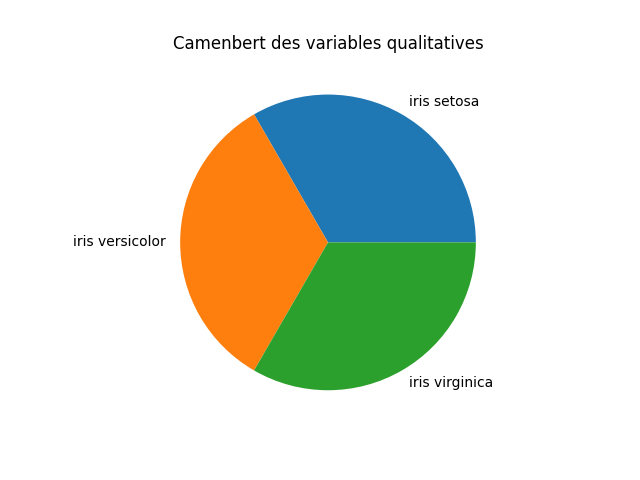
\includegraphics[width=1.1\textwidth]{img/Figure_1.png}
            \caption{\label{fig:camembert}Diagramme camembert des variables qualitatives}  
    \end{center}
    \end{minipage}\hfill
    \begin{minipage}{.48\linewidth}
        \begin{center}
                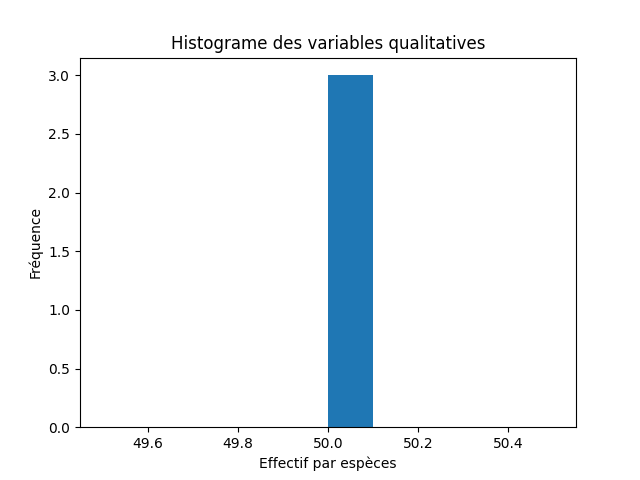
\includegraphics[width=1.1\textwidth]{img/Figure_2.png}
                \caption{\label{fig:histogramme_var-qualitatives}Histogramme des variables qualitatives}  
        \end{center}
    \end{minipage}
\end{figure}

\begin{lstlisting}[style=myPython, caption=Code Python pour tracer le diagramme camenbert et l'histogramme, frame=lines]
nb_species = np.array([iris_setosa, iris_versicolor, iris_virginica])
plt.pie(nb_species, labels=["iris setosa", "iris versicolor", "iris virginica"])
plt.title("Camenbert des variables qualitatives")
plt.show()

plt.hist(nb_species)
plt.title("Histograme des variables qualitatives")
plt.show()
\end{lstlisting}


\subsection{Étude de la variable petalLength}
\subsubsection*{Première approche : graphique}

\vspace{.2cm}

\noindent
\textbf{Question~7~:} Tracer l’histogramme en fréquences et l’histogramme des fréquences cumulées. Faire varier le nombre d’intervalles de l’histogramme.

\vspace{.2cm}

\begin{figure}[!h]
    \centering
    \begin{minipage}{.48\linewidth}
        \begin{center}
            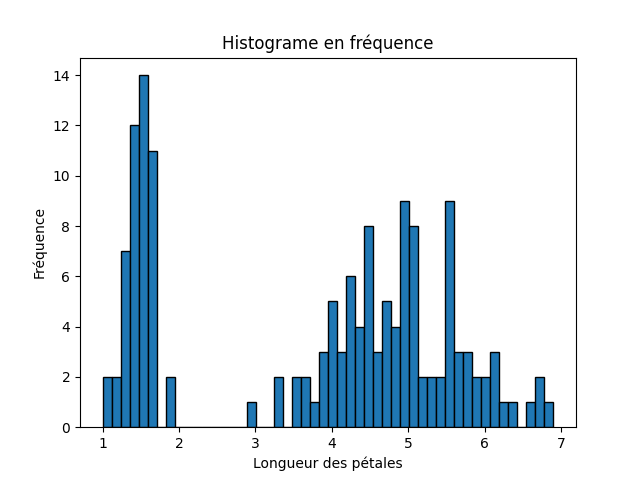
\includegraphics[width=1.1\textwidth]{img/Figure_3.png}
            \caption{\label{fig:histogramme_freq-petalLength}histogramme en fréquences de la variable petalLength}  
    \end{center}
    \end{minipage}\hfill
    \begin{minipage}{.48\linewidth}
        \begin{center}
            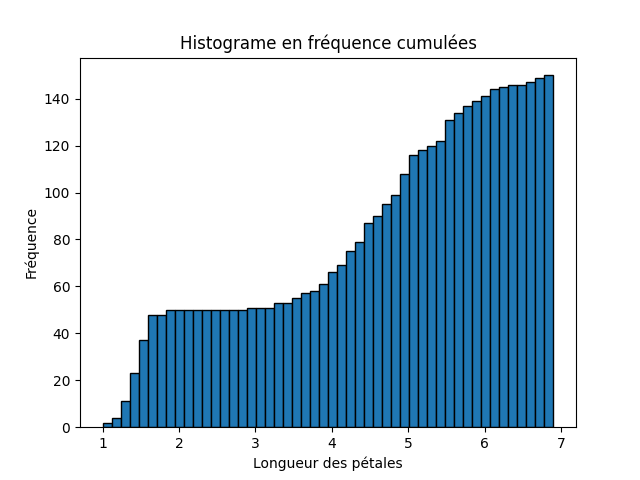
\includegraphics[width=1.1\textwidth]{img/Figure_4.png}
            \caption{\label{fig:histogramme_freq-petalLength-cumul}histogramme en fréquences cumulées de la variable petalLength}  
        \end{center}
    \end{minipage}
\end{figure}

\begin{lstlisting}[style=myPython, caption=Code python pour tracer les histogrammes, frame=lines]
n, x, _ = plt.hist(petallength, 50, edgecolor='black')
plt.title("Histograme en fréquence")
plt.show()

n_cumul, _, _ = plt.hist(petallength, 50, cumulative=True, edgecolor='black')
plt.title("Histograme en fréquence cumulées")
plt.show()
\end{lstlisting}

\vspace{.5cm}


\noindent
\textbf{Question~8~:} Décrire les caractéristiques de l’histogramme et analyser ces caractéristiques en fonction du nombre de classes.
\vspace{.3cm}

On remarque sur l'histogramme en fréquence qu'une majorité des longueurs de pétale est située entre 1 et 2~cm. Si l'on tient compte du nombre de classes, alors on peut penser à deux cas différents~: 
\begin{enumerate}
    \item Le premier serait que deux des trois classes ont majoritairement une longueur de pétale qui varie entre 1 et 2~cm. Dans ce cas, la troisième espèce a une longueur de pétale qui varie entre 3 et 7~cm.
    \item Le second cas serait qu'une des espèces a une longueur de pétale qui varie beaucoup moins que les deux autres. Par exemple l'espèce~1 varie entre 1 et 2~cm, tandis que l'espèce~2 et 3 varie entre 3 et 7~cm. Si l'on suit une 
          logique de probabilité, il est donc évident que l'effectif des longueurs de pétale entre 1 et 2~cm soit plus important puisqu’il y a le même nombre d'effectifs dans chaque espèce et que l'intervalle est plus faible.
\end{enumerate}

\vspace{.2cm}

Le cas numéro~2 semble le plus évident. Si l’on regarde l'histogramme en fréquence cumulé, on constate que le nombre d'effectifs augmente de 2/3 quand le pétale mesure entre 4 et 7~cm.\\
Grâce à l'histogramme en fréquences et l'histogramme en fréquences cumulées on peut conclure qu'une des espèces à une longueur de pétale plus petite que les deux autres, mais qui varie également beaucoup moins


\clearpage

\noindent
\textbf{Question~9~:} Tracer la boite à moustaches (boxplot) et rappeler les différents éléments la constituant.

\begin{figure}[!h]
    \begin{center}
        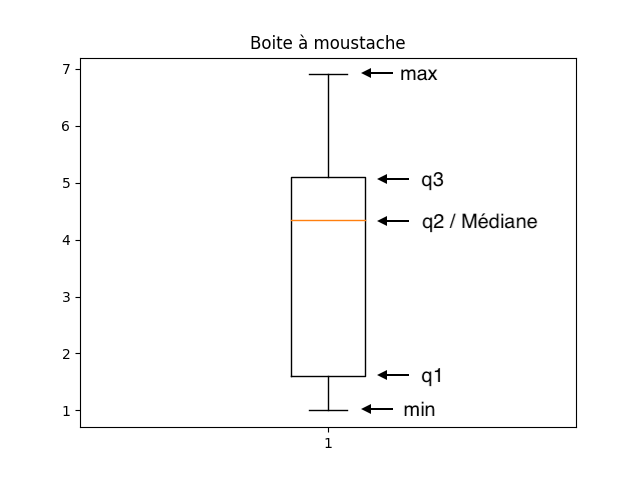
\includegraphics[width=.6\textwidth]{img/Figure_5.png}
        \caption{\label{fig:boite_moustache}Boite à moustache de la variable petalLength}  
    \end{center}
\end{figure}


\begin{lstlisting}[style=myPython, caption=Code Python pour tracer la boite à moustache, frame=lines]
plt.boxplot(petallength)
plt.title("Boite à moustache")
plt.show()
\end{lstlisting}

\vspace{.5cm}




\subsubsection*{Deuxième approche~: résumés numériques}
\vspace{.2cm}

\noindent
\textbf{Question~10~:} Calculer les résumés numériques de localisation (moyenne et médiane) et ceux de dispersion~: (écart-type, variance et quartiles). Retrouver en particulier, les valeurs des éléments de la boite à moustache.
\vspace{.2cm}


\begin{enumerate}
    \item \textbf{Formules utilisées~:}
        \begin{figure}[!h]
            \centering
            \begin{minipage}{.49\linewidth}
                \begin{itemize}
                    \item[--] Moyenne~: 
                        \begin{equation}
                            xn = \frac{1}{n} \sum_{i=0} ni.xi
                        \end{equation}

                    \item[--] Variance~: 
                        \begin{equation}
                            s^2_{n-1} = \frac{1}{n-1} \sum_{i=0} ni(xi - xn)^2
                        \end{equation}
                \end{itemize}
            \end{minipage}\hfill\vline
            \begin{minipage}{.49\linewidth}
                \begin{itemize}
                    \item[--] Médian~:
                        \begin{equation}
                            m=\text{valeur de } x \text{ à la position } \frac{n_{cumul}}{2}
                        \end{equation}

                    \item[--] Écart-type~:
                        \begin{equation}
                            s_{n-1} = \sqrt{s^2_{n-1}}
                        \end{equation}
                \end{itemize}
            \end{minipage}
        \end{figure}

        \begin{itemize}
            \item[--] Quartiles~:
                \begin{gather}
                        q1 = \text{valeur de } x \text{ à la position } \frac{n_{cumul}}{4} \\
                        q2 = m \\
                        q3 = \text{valeur de } x \text{ à la position } \frac{3*n_{cumul}}{4} 
                \end{gather}   
        \end{itemize}

        \clearpage

    \item \textbf{Valeurs obtenues~:}
    
        \vspace{.2cm}

        \begin{center}
            \begin{tabular}{| c |  c | c |}
                \hline
                \multirow{ 2}{*}{\textbf{Résumés numériques de localisation}} & moyenne & 3.701 \\ \cline{2-3}
                                                                    & médian  & 4.186 \\ \hline
                \multirow{ 5}{*}{\textbf{Résumés numériques de dispersion}}   & écart-type & 1.756 \\ \cline{2-3}
                                                                    & variance  & 3.084 \\ \cline{2-3}
                                                                    & q1  & 1.472 \\ \cline{2-3}
                                                                    & q2  & 4.186 \\ \cline{2-3}
                                                                    & q3  & 4.894 \\ \hline
            \end{tabular}
        \end{center}

        \vspace{.5cm}

    \item \textbf{Valeurs reportées sur les graphiques~:}
            \begin{figure}[!h]
                \centering
                \begin{minipage}{.48\linewidth}
                    \begin{center}
                        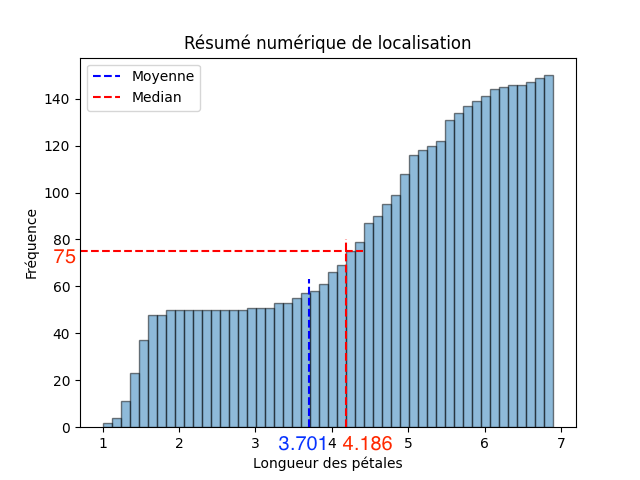
\includegraphics[width=1.1\textwidth]{img/Figure_6.png}
                        \caption{\label{fig:histogramme_freq-petalLength}histogramme en fréquences de la variable petalLength}  
                    \end{center}
                \end{minipage}\hfill
                \begin{minipage}{.48\linewidth}
                    \begin{center}
                        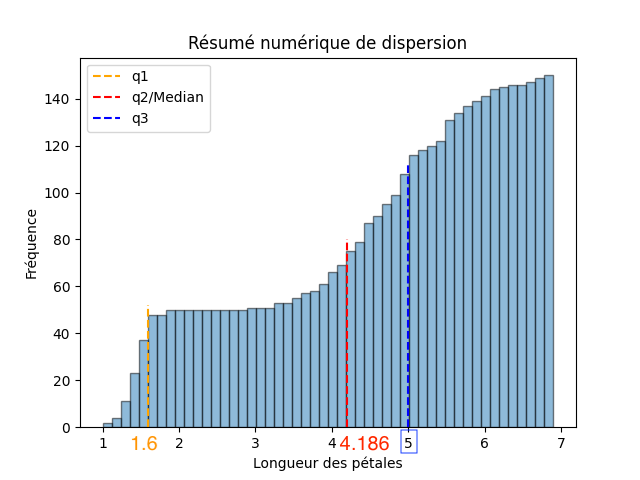
\includegraphics[width=1.1\textwidth]{img/Figure_7.png}
                        \caption{\label{fig:histogramme_freq-petalLength-cumul}histogramme en fréquences cumulées de la variable petalLength}  
                    \end{center}
                \end{minipage}
            \end{figure}
            
            \begin{figure}[!h]
                \begin{center}
                    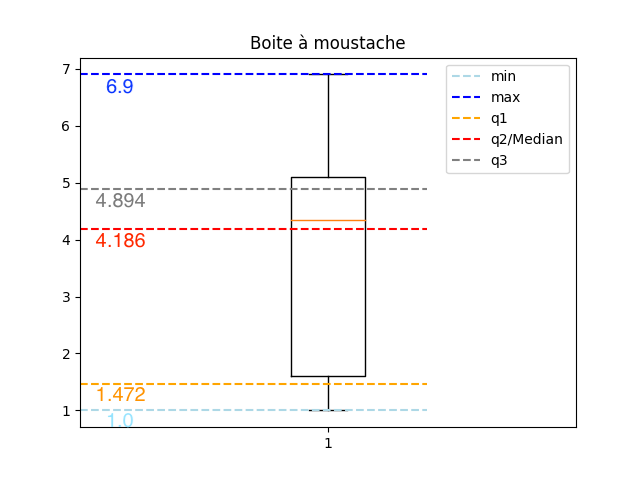
\includegraphics[width=.6\textwidth]{img/Figure_8.png}
                    \caption{\label{fig:boite_moustache}Boite à moustache de la variable petalLength}  
                \end{center}
            \end{figure}

            
    \clearpage


    \item \textbf{Code python~:}
    
    \vspace{.2cm}

    
\begin{lstlisting}[style=myPython, caption=Code python pour le résumé numérique, frame=lines]
def mean(n, x):
    n_max = len(df.values)
    res = 0
    for i in range(len(n)):
        res += (n[i] * x[i])
    ret = (1 / n_max) * res

    return round(ret, 3)

def median(n, x):
    n_median_index = np.where(n == (len(df.values) / 2))

    return float(x[n_median_index])

def variance(n, x, mean):
    n_max = len(df.values)
    res = 0
    for i in range(len(n)):
        res += n[i] * (x[i] - mean) ** 2
    ret = (1 / (n_max - 1)) * res

    return round(ret, 3)

def ecart_type(var):
    return round(np.sqrt(var), 3)

def quartiles(n, x):
    res = x[np.where(n < len(df.values) / 4)]
    q1 = res[-1]

    res = x[np.where(n < (3 * len(df.values)) / 4)]
    q3 = res[-1]

    q2 = median(n_cumul, x)

    return q1, q2, q3

print("RESUME NUMERIQUE DE LOCALISATION :")
print("Moyenne de petallenght:", mean(n, x))
print("Median de petallenght:", median(n_cumul, x), end="\n\n")

q1, q2, q3 = quartiles(n_cumul, x)
print("RESUME NUMERIQUE DE DISPERSION :")
print("Ecart-Type:", ecart_type(variance(n, x, mean(n, x))))
print("Variance:", variance(n, x, mean(n, x)))
print("Quartiles:", '\tq1 =', q1, '\tq2 =', q2, '\tq3 =', q3)
\end{lstlisting}

\begin{lstlisting}[style=myLog, caption=Résultat numérique du code python, frame=lines]
RESUME NUMERIQUE DE LOCALISATION :
Moyenne de petallenght: 3.701
Median de petallenght: 4.186

RESUME NUMERIQUE DE DISPERSION :
Ecart-Type: 1.756
Variance: 3.084
Quartiles: 	q1 = 1.472 	q2 = 4.186 	q3 = 4.894
\end{lstlisting}


\end{enumerate}








\end{document}